\listfiles

\documentclass[a4paper,ngerman,12pt,bibtotoc]{scrartcl}

\usepackage[utf8]{inputenc}

\usepackage[ngerman]{babel}
\addto\captionsngerman{\renewcommand\tablename{Tafel}}

\usepackage{amsmath, amsthm, amssymb, stmaryrd, color, graphicx, mathtools}
\usepackage{setspace}
\usepackage{bussproofs}
\usepackage{array}
\usepackage{booktabs}
\usepackage{comment}
\usepackage{textcomp}
\usepackage{stmaryrd}

\usepackage[protrusion=true,expansion=true]{microtype}

\usepackage{lmodern}
\usepackage{tabto}

\usepackage[backend=bibtex,style=alphabetic]{biblatex}
\usepackage[babel]{csquotes}
\bibliography{literatur}

\usepackage[all]{xy}

\usepackage[colorlinks=true, linkcolor=blue, urlcolor=blue, citecolor=blue]{hyperref}
\usepackage{cleveref}			%Referenzen mit Name


\setlength\parskip{\medskipamount}
\setlength\parindent{0pt}

\theoremstyle{definition}
\newtheorem{defn}{Definition}[section]
\newtheorem{axiom}[defn]{Axiom}
\newtheorem{bsp}[defn]{Beispiel}

\theoremstyle{plain}

\newtheorem{prop}[defn]{Proposition}
\newtheorem{motto}[defn]{Motto}
\newtheorem{ueberlegung}[defn]{Überlegung}
\newtheorem{lemma}[defn]{Lemma}
\newtheorem{kor}[defn]{Korollar}
\newtheorem{hilfsaussage}[defn]{Hilfsaussage}
\newtheorem{satz}[defn]{Satz}

\theoremstyle{remark}
\newtheorem{erin}[defn]{Erinnerung}
\newtheorem{bem}[defn]{Bemerkung}
\newtheorem{beob}[defn]{Beobachtung}
\newtheorem{aufg}[defn]{Aufgabe}

\clubpenalty=10000
\widowpenalty=10000
\displaywidowpenalty=10000

\newcommand{\xra}[1]{\xrightarrow{#1}}
\newcommand{\lra}{\longrightarrow}
\newcommand{\lhra}{\ensuremath{\lhook\joinrel\relbar\joinrel\rightarrow}}
\newcommand{\thlra}{\relbar\joinrel\twoheadrightarrow}

\newcommand{\brak}[1]{\llbracket {#1} \rrbracket}

\newcommand{\ZZ}{\mathbb{Z}}
\newcommand{\QQ}{\mathbb{Q}}
\newcommand{\RR}{\mathbb{R}}
\newcommand{\CC}{\mathbb{C}}
\newcommand{\NN}{\mathbb{N}}
\newcommand{\PP}{\mathbb{P}}
\renewcommand{\aa}{\mathfrak{a}}
\newcommand{\bb}{\mathfrak{b}}
\newcommand{\pp}{\mathfrak{p}}
\newcommand{\mm}{\mathfrak{m}}
\newcommand{\I}{\mathcal{I}}
\newcommand{\J}{\mathcal{J}}
\newcommand{\C}{\mathcal{C}}
\newcommand{\D}{\mathcal{D}}
\newcommand{\E}{\mathcal{E}}
\newcommand{\F}{\mathcal{F}}
\newcommand{\G}{\mathcal{G}}
\newcommand{\U}{\mathcal{U}}
\renewcommand{\I}{\mathcal{I}}
\renewcommand{\P}{\mathcal{P}}
\renewcommand{\O}{\mathcal{O}}
\newcommand{\Hom}{\mathrm{Hom}}
\newcommand{\Ouv}{\mathrm{Ouv}}
\newcommand{\res}{\mathrm{res}}
\newcommand{\Sh}{\mathrm{Sh}}
\newcommand{\PSh}{\mathrm{PSh}}
\newcommand{\Bohr}{\mathrm{Bohr}}
\newcommand{\pt}{\mathrm{pt}}
\newcommand{\ev}{\mathrm{ev}}
\newcommand{\id}{\mathrm{id}}
\newcommand{\Id}{\mathrm{Id}}
\newcommand{\freist}{\underline{\ \ }}
\newcommand{\ul}[1]{\underline{#1}}
\newcommand{\csalgebra}{C\textsuperscript{*}\kern-.1ex-Algebra}
\newcommand{\csalgebren}{C\textsuperscript{*}\kern-.1ex-Alge\-bren}
\DeclareMathOperator{\colim}{colim}
\DeclareMathOperator{\Ob}{Ob}
\DeclareMathOperator{\ggT}{ggT}
\DeclareMathOperator{\im}{im}
\DeclareMathOperator{\Quot}{Quot}
\DeclareMathOperator{\Spec}{Spec}
\DeclareMathOperator{\interior}{int}
\newcommand{\op}{\mathrm{op}}
\newcommand{\Set}{\mathrm{Set}}
\newcommand{\Grp}{\mathrm{Grp}}
\newcommand{\Vect}[1]{{#1\text{-}\mathrm{Vect}}}
\newcommand{\AbGrp}{\mathrm{AbGrp}}
\newcommand{\Ring}{\mathrm{Ring}}
\newcommand{\Cat}{\mathrm{Cat}}
\newcommand{\Funct}{\mathrm{Funct}}
\newcommand{\Eins}{\mathbf{1}}
\newcommand{\Man}{\mathrm{Man}}
\newcommand{\Top}{\mathrm{Top}}
\newcommand{\seq}[1]{\mathrel{\vdash\!\!\!_{#1}}}
\renewcommand{\_}{\mathpunct{.}\,}
\newcommand{\?}{\,{:}\,}

\newcommand{\Alg}{\ensuremath{\textsc{alg}}}
\newcommand{\Opt}{\ensuremath{\textsc{opt}}}
\newcommand{\Robl}{\overline{\mathcal{R}}_\mathrm{OBL}}
\newcommand{\EE}{\mathbf{E}}
\newcommand{\si}{\tilde{\imath}}		%Sattelpunkt i
\newcommand{\sj}{\tilde{\jmath}}		%Sattelpunkt j
\newcommand{\sx}{\tilde{x}}		%Sattelpunkt i
\newcommand{\sy}{\tilde{y}}		%Sattelpunkt j
\renewcommand{\sp}{\tilde{p}}		%Sattelpunkt i
\newcommand{\sq}{\tilde{q}}		%Sattelpunkt j
\newcommand{\sjn}{\sigma_j^n}
\newcommand{\sjm}{\sigma_j^m}
\newcommand{\Hf}{H}
\newcommand{\EH}{\boldsymbol{H}}

\newcommand{\ZPNS}{Zwei-Personen-Nullsummenspiel }

\newcommand{\defeq}{\vcentcolon=}
\newcommand{\defequiv}{\vcentcolon\equiv}

\renewcommand*\theenumi{\alph{enumi}}
\renewcommand{\labelenumi}{(\theenumi)}

\newcommand\subsubsubsection[1]{\subsubsection*{#1}}
\definecolor{grey}{rgb}{0.7,0.7,0.7}

\setcounter{tocdepth}{2}

\newenvironment{indentblock}{%
	\list{}{\leftmargin\leftmargin}%
	\item\relax
}{%
\endlist
}



\begin{document}
	\author{Lukas Graf}
	\title{Online-Optimierung als \ZPNS und Yaos Prinzip}
	\date{\today}
	
	\selectlanguage{ngerman}
	\thispagestyle{empty}
	
	\maketitle

	\section*{Einführung}
	
	Stellen wir uns vor wir haben ein bestimmtes Online-Optimierungsproblem gegeben und fragen uns wie \glqq schwer\grqq{} dieses ist. Eine natürliche Weise dies zu beurteilen wäre dann sich zu fragen, wie gut ein bester Online-Algorithmus für dieses Problem ist, d.h. welche Kompetitivität wir mit diesem besten Algorithmus erreichen können.
	
	Da wir letzteren im Allgemeinen aber wohl nicht von Vornherein kennen werden, wäre es etwas viel verlangt diese Kompetitivität exakt zu bestimmen. Stattdessen wollen wir versuchen, obere und untere Schranken für die Kompetitivität des bestmöglichen Online-Algorithmus zu finden. 
	
	Den einfachen Fall bilden hierbei offenbar die oberen Schranken: Dazu müssen wir uns nur einen beliebigen Online-Algorithmus vorgeben und dessen Güte bestimmen. Die Kompetitivität eines besten Online-Algorithmus kann dann höchstens so groß sein, wie die des soeben gewählten Algorithmus. Schwieriger ist dagegen das Finden unterer Schranken: Wie sollen wir Aussagen darüber treffen, welche Kompetitivität kein Online-Algorithmus unterschreiten kann (ohne dazu alle denkbaren Online-Algorithmen auszuprobieren)?
	
	Eine Antwort darauf liefert ein von Andrew Yao entwickeltes Prinzip (\cite*[Theorem 1]{Yao}), welches auf der Idee basiert Online-Optimierungsprobleme als Nullsummenspiel zwischen zwei Personen aufzufassen: Dem Online-Spieler, der versucht einen möglichst guten Online-Algorithmus zu finden, und dem Offline-Spieler, dessen Ziel es ist eine Anfragesequenz zu finden, auf der der gewählte Online-Algorithmus im Verhältnis zum optimalen Offline-Algorithmus möglichst schlecht abschneidet.
	
	Dank dieser Betrachtungsweise lassen sich dann Erkenntnisse aus der Spieltheorie (und hier insbesondere von Neumanns Minimax-Theorem) auf die Online-Optimierung übertragen. Dadurch werden wir nicht nur tatsächlich einen Weg finden untere Schranken für die Kompetitivität zu bestimmen, sondern wir können sogar zeigen, dass auf diese Weise (wenigstens theoretisch) immer eine solche untere Schranke gefunden werden kann, die mit der stärksten obersten Schranke zusammenfällt (und somit gerade die Kompetitivität eines besten Online-Algorithmus festlegt).
	
	Die vorliegende Ausarbeitung orientiert sich im Wesentlichen an Kapitel 8 des Buches \citetitle{OCCA} von \citeauthor{OCCA} (\cite{OCCA}). Der Beweis von Yaos Prinzip verwendet darüber hinaus einige Vereinfachungen aus Kapitel 5 des Skriptes \citetitle{OO} von \citeauthor{OO} (\cite{OO}).
	

	\section{\ZPNS}
	
%	\begin{bsp}
%		Am Ende des Semesters werden verschiedene Seminare für das kommende Semester angeboten. 
%	\end{bsp}
	
	Ein Zwei-Personen Spiel ist im Wesentlichen eine (endliche) Abfolge von Entscheidungen zweier Spieler (man denke beispielsweise an Schere-Stein-Papier, Tic-Tac-To, Schach, ...). Um daraus ein Nullsummenspiel zu machen, müssen wir dann außerdem für jeden denkbaren Spielausgang einen gewissen Betrag festlegen, den Spieler 1 an Spieler 2 zahlen muss (oder umgekehrt - letzteres werden wir im Folgenden der Einfachheit halber immer als negative Auszahlung von Spieler 1 an Spieler 2 auffassen). 
	
	\begin{bsp}\label{bsp:teil1}
		Ein einfaches Spiel könnte beispielsweise so aussehen: 
		
		Unser Gegenspieler denkt sich eine endliche Folge natürlicher Zahlen aus. Dann zählt er nacheinander die Zahlen dieser Folge auf, bis wir \glqq Stopp\grqq{} sagen (oder die Folge zu Ende ist). Danach verrät unser Gegenspieler, was die kleinste Zahl in seiner Folge war und wir zahlen ihm die Differenz der Zahl, bei der wir \glqq Stopp\grqq{} gesagt haben, und dem Eineinhalbfachen der kleinsten Zahl der Folge.
		
		\begin{figure}[h]
			\centering
			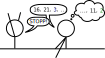
\includegraphics[width=0.45\linewidth]{../Bilder/Comic}
			\caption{\small Finde die kleinste Zahl!}
			\label{fig:Comic}
		\end{figure}

		
		Unser Ziel ist es folglich bei einer Zahl \glqq Stopp\grqq{} zu sagen, die möglichst nahe an der kleinsten Zahl der Folge liegt (idealerweise höchstens 1,5-mal so groß ist, damit wir auch Gewinn machen).
		
		Eine naheliegende Fragestellung wäre dann, welche Strategie in diesem Spiel besonders erfolgversprechend ist, oder auch, ob es überhaupt eine Strategie gibt, mit der wir einen sicheren Gewinn machen können.
	\end{bsp}
	
	Um nun leichter verschiedene Spielabläufe vergleichen zu können, wollen wir außerdem davon ausgehen, dass die beiden Spieler ihre Entscheidungen nicht erst unter dem Spiel \glqq spontan\grqq{} treffen, sondern bereits zu Beginn des Spiels für jede denkbare Entscheidungssituation\footnote{Jede solche Entscheidungssituation wird dabei festgelegt durch alle Informationen, die dem jeweiligen Spieler zu diesem Zeitpunkt bekannt sind (also bspw. zuvor bereits getroffene Entscheidungen)} festlegen, welche Entscheidung sie in dieser treffen würden. Alle diese Festlegungen zusammen bezeichnen wir dann als \emph{reine Strategien} der beiden Spieler.
	
	Damit lässt sich ein (endliches) \ZPNS wie folgt beschreiben:
	
	\begin{defn}
		Ein \emph{(endliches) \ZPNS} ist gegeben durch
		\begin{itemize}
			\item eine Menge von \emph{reinen Strategien} $\{s^1_i \mid i \in I\}$ für Spieler 1 (indiziert durch eine endliche Menge $I$),
			\item eine Menge von \emph{reinen Strategien} $\{s^1_j \mid j \in J\}$ für Spieler 2 (indiziert durch eine endliche Menge $J$)
			\item und eine \emph{Auszahlungsfunktion} $\Hf: I \times J \to \mathbb{R}$ für Spieler 1.
		\end{itemize}
		Wählen also Spieler 1 und 2 die reinen Strategien $s^1_i$ bzw. $s^2_j$, so zahlt Spieler 1 nach Ende des Spiels $\Hf(i,j)$ an Spieler 2. Offenbar ist nun das Ziel von Spieler 1 die Auszahlungsfunktion $\Hf$ durch die Wahl seiner Strategie zu minimieren (Spieler 1 ist \emph{Kostenminimierer}), während Spieler 2 versucht $\Hf$ zu maximieren (Spieler 2 ist \emph{Gewinnmaximierer}).
	\end{defn}
	
	\begin{bem}
		Die Kostenfunktion (und damit effektiv das gesamte Spiel) lässt sich gut als Matrix darstellen, deren Zeilen den reinen Strategien von Spieler 1 und deren Spalten den reinen Strategien von Spieler 2 entsprechen:
		\[\begin{array}{l||c|c|c}
					& \dots & s^2_j	& \dots \\\hline\hline
			 \vdots & 		&		&		\\\hline
			 s^1_i	&		&\Hf(i,j)&		\\\hline
			 \vdots &		&		&			
		\end{array}\]
		Entsprechend wird Spieler 1 dann als \glqq Zeilenspieler\grqq{} und Spieler 2 als \glqq Spaltenspieler\grqq{} bezeichnet. Die Wahl einer reinen Strategie entspricht sodann der Wahl einer Zeile $i$ bzw. Spalte $j$. Daher werden wir im Folgenden oft nicht mehr zwischen der Strategie $s^1_i$ und dem Index dieser Strategie $i$ unterscheiden und direkt von der \glqq Strategie $i$\grqq{} sprechen.
	\end{bem}	

	\begin{defn}
		Ein Online-Optimierungsproblem (mit blindem Offline-Gegenspieler) können wir nun wie folgt als \ZPNS auffassen:
		\begin{itemize}
			\item Spieler 1 ist der Online-Spieler und seine reinen Strategien entsprechen den zur Verfügung stehenden deterministischen Algorithmen $\{\Alg_i \mid i \in I\}$.
			\item Spieler 2 ist der Offline-Gegenspieler und seine reinen Strategien entsprechend den zulässigen endlichen Anfragesequenzen $\{\sigma_j \mid j \in J\}$.
			\item Als Auszahlungsfunktion wählen wir für eine fest gewählte Konstante $c \geq 1$:
			\[\Hf_c(i,j) := \Alg_i(\sigma_j) - c\cdot\Opt(\sigma_j)\]
		\end{itemize}
	\end{defn}
	
	\begin{bem}
		Damit wir auf diesem Weg tatsächlich ein \emph{endliches} \ZPNS erhalten, müssen wir also voraussetzen, dass auch das ursprüngliche Optimierungsproblem in einem gewissen Sinne endlich ist: Es darf nur endlich viele Anfragesequenzen geben und können nur endlich viele deterministische Algorithmen zur Auswahl stehen.
		
		Bis einschließlich \Cref{sec:YaosPrinzip} werden wir nun ausschließlich solche endlichen Online-Optimierungsprobleme betrachten.
	\end{bem}
	
	\begin{beob}
		Diese Auszahlungsfunktion erlaubt uns folgende Interpretation: Ein Algorithmus $\Alg_i$ ist genau dann $c$-kompetitiv, wenn $\Hf_c$ für alle möglichen Anfragesequenzen kleiner oder gleich 0 ist.\footnote{Für endliche Online-Optimierungsprobleme betrachten wir hier ausschließlich \emph{strikte} $c$-Kompetitivität. Durch Zulassen einer additiven Konstante $\alpha$ könnten wir sonst trivialerweise immer jede beliebige Kompetitivität erreichen (durch Setzen von $\alpha$ auf die maximalmöglichen Kosten des gerade betrachteten Online-Algorithmus). }
	\end{beob}
	
	\begin{bsp}\label{bsp:Teil2}
		Betrachten wir noch einmal das Spiel aus \Cref{bsp:teil1}, so sehen wir, dass dieses im Grunde bereits die Modellierung eines Online-Optimierungsproblems ist: 
		
		Die Anfragesequenzen\footnote{Um die Endlichkeitsbedingung zu erfüllen sollten wir die Menge der Anfragesequenzen hier noch weiter einschränken - etwa indem wir fordern, dass diese Länge $k$ haben müssen und nur Zahlen aus $\{1, \dots, n\}$ enthalten dürfen (für feste $k$ und $n$). Die Menge aller deterministischen Algorithmen ist dann automatisch endlich (unter der - sicher sinnvollen - Annahme, dass wir zwei Algorithmen nur als verschieden ansehen wollen, wenn sie auf wenigstens einer Folge zu unterschiedlichen Ergebnissen führen)} sind die Folgen natürlicher Zahlen und unsere Aufgabe ist es die kleinste Zahl (bzw. zumindest eine möglichst kleine) darin zu finden. Es handelt sich hierbei auch tatsächlich um ein Online-Problem, da wir die Sequenz nur stückweise erfahren und immer sofort eine Entscheidung treffen müssen (ist das die kleinste Zahl oder warten wir noch auf eine kleinere?).
		
		Das beschriebene Auszahlungsverfahren (wir zahlen unsere Zahl - $1,5\times$ die kleinste Zahl an Spieler 2) entspricht gerade der Wahl $c=1,5$ in der oben beschriebenen Auszahlungsfunktion (der optimale Offline-Algorithmus ist sicher immer in der Lage die tatsächlich kleinste Zahl der Folge zu finden).
		
		Unsere Suche nach einer guten Spielstrategie übersetzt sich damit in die Suche nach einem guten Online-Algorithmus. Die Frage, ob wir erwarten können in diesem Spiel Gewinn zu machen, wird zur Frage, ob es für dieses Problem einen 1,5-kompetitiven Online-Algorithmus gibt.
	\end{bsp}
	
	Anstatt vor jedem Spiel eine neue Strategie wählen zu müssen, wollen wir den nun Spielern auch erlauben ihre Strategie zu Beginn des Spiels zufällig zu bestimmen. Dazu legen die Spieler eine Wahrscheinlichkeitsverteilung über den ihnen zur Verfügung stehenden reinen Strategien fest. Die tatsächliche Strategie wird dann zu Beginn des Spiels gemäß der Verteilung zufällig ausgewählt.
	
	Da die Wahl der Strategien und damit auch die Spielabläufe nun ein zufälliges Element beinhalten, können wir dann nicht mehr von \glqq der Auszahlung\grqq{} sprechen, sondern sollten die erwartete Auszahlung betrachten, d.h. den Erwartungswert gebildet über der Auszahlungsfunktion.
	
	\begin{defn}Für ein \ZPNS definieren wir:	
		\begin{itemize}
			\item Eine \emph{gemischte Strategie für Spieler 1} ist eine Wahrscheinlichkeitsverteilung $p$ über den ihm zur Verfügung stehenden reinen Strategien. Wir können damit $p$ als durch $I$ indizierten Vektor $(p_i)_{i\in I}$ auffassen, wobei $p_i$ die Wahrscheinlichkeit bezeichnet, dass die Strategie $s_i^1$ ausgewählt wird.
			\item Analog definieren wir eine \emph{gemischte Strategie für Spieler 2} als $(q_j)_{j\in J}$.
			\item Für zwei gemischte Strategien $p$ und $q$ ist die \emph{erwartete Auszahlung} dann:
			\[\EH(p,q) := \EE_{p,q}\left[\Hf(i,j)\right] := \sum_{i\in I, j\in J} p_i q_j \Hf(i,j)\]
		\end{itemize}
	\end{defn}
	
	\begin{bem}\label{bem:SpielAeq}
		Man könnte nun vermuten, dass die Einschränkung nur einmal zu Beginn den Zufall entscheiden zu lassen, und danach deterministisch zu spielen eine recht starke Einschränkung ist. Insbesondere dann, wenn wir gerade ein Online-Optimierungsproblem modellieren wollen - man kann sich schließlich leicht Algorithmen vorstellen, die auch zur Ausführungszeit noch weitere Zufallsentscheidungen treffen. Im Allgemeinen ist dies auch so.
		
		Es gibt aber bestimmte Klassen von Spielen, für die das nicht so ist (in denen es also zu jeder denkbaren Strategie auch eine mindestens ebenso gute gemischte Strategie nach obiger Definition gibt). Eine solche Klasse bilden die Spiele mit perfektem Gedächtnis (siehe \cite[Theorem 6.3]{OCCA}). Für Online-Optimierungsprobleme ist die entsprechende Bedingung dabei schon dann erfüllt, wenn wir davon ausgehen, dass die Algorithmen (sowohl Online als auch Offline) über unbegrenzten Speicher verfügen können - was wir im Folgenden auch tun wollen.
	\end{bem}
	
	\begin{bem}
		Auf die als Nullsummenspiele modellierten Online-Optimierungs"-pro"-ble"-me überträgt sich die Einführung des Zufalls wie folgt:
		\begin{itemize}
			\item Eine gemischte Strategie $p$ von Spieler 1 entspricht hier einem randomisierten Algorithmus $\Alg_p$, der zu Beginn einmal anhand der Verteilung $p$ ein zufälliges $i$ aus $I$ zieht und dann den entsprechenden deterministischen Algorithmus $\Alg_i$ ausführt.\footnote{Unter der in \Cref{bem:SpielAeq} beschriebenen Annahme erhalten wir auf diesem Weg effektiv \emph{alle} randomisierten Online-Algorithmen (bzw. zumindest jeweils äquivalente). Wir können mit dieser Modellierung daher tatsächlich Aussagen über alle randomisierten Online-Algorithmen treffen. 
				
			Umgekehrt heißt dies allerdings auch: Untersuchen wir ein Online-Optimierungsproblem, in dem besagte Annahme verletzt ist (in dem also der interne Speicherplatz der Algorithmen begrenzt ist), so ist die Gültigkeit der hier gezeigten Aussagen nicht mehr gewährleistet!}
			\item Einer gemischten Strategie von Spieler 2 entspricht, dass die Anfragesequenz zu Beginn zufällig gemäß einer Wahrscheinlichkeitsverteilung über allen möglichen Anfragesequenzen $\{\sigma_j \mid j \in J\}$ gewählt wird.
			\item Die erwartete Auszahlungsfunktion ist dann gegeben durch:
				\[\EH_c(p,q) := \EE_{p,q}\left[\Alg_i(\sigma_j) - c\cdot\Opt(\sigma_j)\right] = \EE_{p,q}\left[\Alg_i(\sigma_j)\right] - c\cdot\EE_{q}\left[\Opt(\sigma_j)\right]\]
			Beachte, dass das Ergebnis des optimalen Offline-Algorithmus natürlich unabhängig von der Zufallsentscheidung des Online-Algorithmus ist.
		\end{itemize}
	\end{bem}
	
	\begin{beob}
		Die gemischten Strategien beinhalten insbesondere auch wieder alle reinen Strategien. Denn wir können jede reine Strategie $k$ mit der Wahrscheinlichkeitsverteilung $e^{(k)} :=(\delta_{k i})_{i\in I}$ identifizieren, die zu 100\% die reine Strategie $k$ auswählt.
	\end{beob}
	
	\begin{beob}
		Auch die erwartete Auszahlungsfunktion lässt sich wieder im Rahmen der Online-Optimierung interpretieren: Ein randomisierter Algorithmus $\Alg_p$ ist genau dann $c$-kompetitiv, wenn $\EH_c$ für alle möglichen (deterministischen!) Anfragesequenzen kleiner oder gleich 0 ist, d.h.
		\begin{equation}\label{eq:ckomKrit}
			\Alg_p \text{ ist } c\text{-komp.} \iff 0 \geq \max_{j\in J} \EH_c(p,e^{(j)}) = \max_{j\in J}\left(\EE_{p}\left[\Alg_i(\sigma_j)\right] - c\cdot\Opt(\sigma_j)\right)
		\end{equation}
		Für einen gegebenen Algorithmus $\Alg_p$ ist damit
			\[c := \max_{j\in J}\frac{\EE_{p}\left[\Alg_i(\sigma_j)\right]}{\left[\Opt(\sigma_j)\right]}\]
		gerade dessen Kompetitivitätsverhältnis.
	\end{beob}
	
	Eine untere Schranke für die Kompetitivität aller Algorithmen in einem gegebenen Online-Optimierungsproblem zu finden ist damit äquivalent dazu ein $c\geq 1$ zu finden, für das wir zeigen können, dass $\max_{j\in J}\left(\EE_{p}\left[\Alg_i(\sigma_j)\right] - c\cdot\Opt(\sigma_j)\right)$ für jede Verteilung $p$ (also jeden randomisierten Online-Algorithmus $\Alg_p$) größer oder gleich 0 ist. Anders gesagt: Wir wollen ein $c\geq 1$ finden, sodass gilt:
	\begin{equation}\label{eq:untereSchranke}
		\min_p\max_{j\in J}\left(\EE_{p}\left[\Alg_i(\sigma_j)\right] - c\cdot\Opt(\sigma_j)\right) \geq 0
	\end{equation}
	
	Dazu wollen wir nun zunächst das analoge Problem im allgemeinen spieltheoretischen Umfeld betrachten:
	
	
	\section{Sattelpunkte und Wert eines Spiels}
	
	Gegeben sei ein beliebiges 2-Personen Nullsummenspiel. Vorausgesetzt beide Spieler spielen absolut rational, welche Auszahlung sollten wir dann erwarten? Oder, etwas schwächer formuliert: Mit welcher Auszahlung können die beiden Spieler bei ausreichend guter Spielweise mindestens rechnen?
	
	Um zu versuchen diese Frage zu beantworten, wollen wir das Spiel nun aus folgender \glqq pessimistischen\grqq{} Sichtweise der beiden Spieler betrachten:
	\begin{itemize}
		\item Spieler 1 versucht seine maximalen Kosten zu minimieren. Daher betrachtet er nun für jede seiner Strategien $p$ den schlimmstmöglichen Fall, also die Auszahlung $\max_q \EH(p,q)$. Seine Strategie wählt er daher so, dass diese größtmögliche Auszahlung möglichst klein wird. Der daraus resultierende Wert
			\[\min_p \max_q \EH(p,q)\]
		ist damit offenbar eine obere Schranke für die kleinste Auszahlung, die Spieler 1 sicherstellen kann.
		\item Analog versucht Spieler 2 die minimalen Kosten für Spieler 1 zu maximieren. Er wählt seine Strategie $q$ daher so, dass die kleinstmögliche Auszahlung $\min_p \EH(p,q)$ möglichst groß wird. Der Wert
			\[\max_q \min_p \EH(p,q)\]
		wird somit zu einer unteren Schranke für die höchste Auszahlung, die Spieler 2 sicherstellen kann.
	\end{itemize}
	
	\begin{bem}
		Alle oben auftauchenden Minima bzw. Maxima sind wohldefiniert, denn die Menge der Wahrscheinlichkeitsverteilungen über den endlichen Mengen $I$ bzw. $J$ ist kompakt und $\EH$ stetig. Also nimmt $\EH$ beide Extremwerte an.
	\end{bem}
	
	\begin{beob}\label{beob:minmaxgeqmaxmin}
		Es ist nun leicht zu sehen, dass allgemein gilt 
			\[\min_p \max_q \EH(p,q) \geq \max_q \min_p \EH(p,q),\]
		d.h. die worst-case Kosten, mit denen Spieler 1 rechnet, sind mindestens so hoch, wie die worst-case Kosten, mit denen Spieler 2 rechnet.
		
	\end{beob}

	\begin{proof}
		Für alle Strategien $\sp$ und $\sq$ gilt sicher, dass die beste Konter-Strategie $q$ von Spieler 2 gegen $\sp$ eine mindestens so hohe Auszahlung liefert wie $\sq$. Ebenso führt die beste Konter-Strategie $p$ von Spieler 1 gegen $\sq$ zu einer höchstens so hohen Auszahlung wie $\sp$. Zusammen erhalten wir also für alle Strategien  $\sp$ und $\sq$:
			\[\max_q\EH(\sp,q) \geq \EH(\sp,\sq) \geq \min_p\EH(p,\sq)\]
		Insbesondere gilt also für alle Strategien $\sp$ und $\sq$
			\[\max_q\EH(\sp,q) \geq \EH(\sp,\sq) \geq \min_p\EH(p,\sq)\]
		und daher auch (bei Wahl der entsprechend besten Stratgien)
			\[\min_p \max_q \EH(p,q) \geq \max_q \min_p \EH(p,q). \qedhere\]
		\end{proof}	
	
	Interessant wäre es nun zu wissen, wann hier sogar Gleichheit gilt - wann also die von Spieler 1 und Spieler 2 durch ihre worst-case-Analysen gefundenen Schranken übereinstimmen. Ist dies nämlich der Fall, so ist der dadurch erhaltene Wert wohl ein guter Kandidat für die Auszahlung, die wir bei optimaler Spielweise beider Spieler erwarten sollten. Wir definieren daher:
	
	\begin{defn}
		Gilt in einem Spiel $\min_p \max_q \EH(p,q) = \max_q \min_p \EH(p,q) =: v$, so bezeichnen wir $v$ als \emph{den Wert des Spiels}.
	\end{defn}
	
	Um nun die Frage zu beantworten, wann diese Gleichheit tatsächlich auftritt, wollen wir noch eine alternative Spielweise betrachten: Spieler 1 wählt zunächst eine beliebige Strategie und verrät diese Spieler 2. Dieser wählt dann seine beste Konterstrategie. Daraufhin (also zum Beispiel im nächsten Spiel) wählt Spieler 1 die Strategie, die den besten Konter zu Spieler 2s Konterstrategie darstellt. Als nächstes passt wieder Spieler 2 seine Strategie an usw.
	
	Eine naheliegende Frage ist dann, ob sich dieses Verfahren jemals stabilisieren kann, d.h. ob es eine Kombination von gemischten Strategien gibt, sodass sich für keinen der beiden Spieler ein weiterer (einseitiger) Strategiewechsel lohnt. Gibt es eine solche Kombination, wollen wir diese als Sattelpunkt bezeichnen:
	
	\begin{defn}
		Ein Tupel $(\sp, \sq)$ von gemischten Strategien heißt \emph{Sattelpunkt}, wenn gilt:
			\[\text{Für alle gemischte Strategien } p, q \text{ gilt}: \EH(\sp,q) \leq \EH(\sp,\sq) \leq \EH(p,\sq)\]
		D.h. in einem Sattelpunkt gilt: Spieler 1 kann die Auszahlung durch einen Strategiewechsel höchstens erhöhen, während Spieler 2 die Auszahlung durch einen Strategiewechsel höchstens senken kann. Eine solche Situation bezeichnet man auch als \emph{Nash-Gleichgewicht}.
	\end{defn}
	
	Offenkundig wäre nun auch die Auszahlung $\EH(\sp,\sq)$ in einem Sattelpunkt ein naheliegender Kandidat für die Auszahlung, die wir bei vernünftiger  Spielweise beider Spieler erwarten können. Und tatsächlich stimmen diese beiden Werte sogar überein, wie folgendes Lemma zeigen wird:
	
	\begin{lemma}\label{lemma:AeqWertSattel}
		Für jedes endliche \ZPNS sind äquivalent: 
		\begin{enumerate}
			\item Das Spiel hat einen Sattelpunkt $(\sp,\sq)$
			\item Das Spiel hat einen Wert, d.h. $\min_p \max_q \EH(p,q) = \max_q \min_p \EH(p,q)$
		\end{enumerate}
	\end{lemma}
	
	\begin{proof}
		\glqq \textit{(a)$\Rightarrow$(b)}\grqq: Ist $(\sp,\sq)$ ein Sattelpunkt, so gilt nach Definition:		
		\begin{alignat*}{9}
						&\forall p,q:	&		& 		&\EH(\sp,q) &\leq \EH(\sp,\sq) \leq &		&		&\EH(p,\sq) \\
			\Rightarrow	&				&		&\max_q	&\EH(\sp,q) &\leq \EH(\sp,\sq) \leq &		&\min_p	&\EH(p,\sq) \\
			\Rightarrow	& 				&\min_p &\max_q	&\EH(p,q)	&\leq \EH(\sp,\sq) \leq &		&\min_p	&\EH(p,\sq) \\
			\Rightarrow	&				&\min_p	&\max_q\,&\EH(p,q) 	&\leq \EH(\sp,\sq) \leq\,&\max_q&\min_p\,&\EH(p,q)
		\end{alignat*}
		Zusammen mit \Cref{beob:minmaxgeqmaxmin} folgt daraus
			\[\min_p\max_q\EH(p,q) = \EH(\sp,\sq) = \max_q\min_p\EH(p,q)\]
		und daher gilt \textit{(b)}.
		
		\glqq \textit{(b)$\Rightarrow$(a)}\grqq: Es gelte $\min_p \max_q \EH(p,q) = \max_q \min_p \EH(p,q) =: v$. Dann gibt es Strategien $\sp$ und $\sq$, an denen das \glqq äußere\grqq{} Minimum bzw. Maximum angenommen wird:
			\[\max_q \EH(\sp,q) = v = \min_p \EH(p,\sq)\]
		Daraus wiederum erhalten wir für beliebige Strategien $p$ und $q$ die folgende Ungleichung:
			\[\EH(\sp,q) \leq v \leq \EH(p,\sq)\]
		Insbesondere gelten also (für alle $p$ und $q$):
			\[\EH(\sp,q) \leq v \leq \EH(\sp,\sq) \text{ und } \EH(\sp,\sq) \leq v \leq \EH(p,\sq)\]
		und damit ist $(\sp,\sq)$ ein Sattelpunkt.
	\end{proof}
	
	\begin{beob}
		Aus dem Beweis zu \glqq \textit{(a)$\Rightarrow$(b)}\grqq{} folgt insbesondere, dass die Auszahlung am Sattelpunkt gerade dem Wert des Spiels entspricht.
	\end{beob}
	
	\begin{bem}
		Beachte, dass alle bisherigen Definition und Aussagen auch genauso für den Fall gelten, dass wir nur reine Strategien erlauben. 
	\end{bem}
	
	\begin{bsp}\label{bsp:Teil3}
		Wir schränken nun \Cref{bsp:Teil2} noch weiter ein, indem wir unserem Gegenspieler nur noch erlauben Folgen der Länge 2 aus den Zahlen 1, 2 und 3 zu bilden. Ein deterministischer Online-Algorithmus ist dann bereits dadurch eindeutig bestimmt, wann er sich für die erste Zahl entscheidet (und wann für die zweite). Bspw. sei also $\Alg_{\{1,3\}}$ der Algorithmus, der sich für die erste Zahl entscheidet, falls diese 1 oder 3 ist und sonst auf die zweite Zahl wartet.
		
		Schreiben wir nun alle möglichen Anfragesequenzen als Spalten und alle deterministischen Algorithmen als Zeilen, so erhalten wir die folgende Tabelle:
		\def\arraystretch{1.5}
		\[\footnotesize\begin{array}{l||c|c|c|c|c|c}
		& 1,2 & 1,3	& 2,1 & 2,3 & 3,1 & 3,2 \\\hline\hline
		\Alg_\emptyset 	& 2/1 & 3/1	& 1/1 & 3/2	& 1/1 & 2/2	\\\hline
		\Alg_{\{1\}}	& 1/1 & 1/1 & 1/1 & 3/2 & 1/1 & 2/2 \\\hline
		\Alg_{\{2\}}	& 2/1 & 3/1 & 2/1 & 2/2 & 1/1 & 2/2 \\\hline
		\Alg_{\{3\}}	& 2/1 & 3/1 & 1/1 & 3/2 & 3/1 & 3/2 \\\hline
		\Alg_{\{1,2\}}	& 1/1 & 1/1 & 2/1 & 2/2 & 1/1 & 2/2 \\\hline
		\Alg_{\{1,3\}}	& 1/1 & 1/1 & 1/1 & 3/2 & 3/1 & 3/2 \\\hline
		\Alg_{\{2,3\}}	& 2/1 & 3/1 & 2/1 & 2/2 & 3/1 & 3/2 \\\hline
		\Alg_{\{1,2,3\}}& 1/1 & 1/1 & 2/1 & 2/2 & 3/1 & 3/2
		\end{array}\]
		Zur Notation der Auszahlung verwenden wir hierbei folgende Konvention: Anstatt den tatsächlichen Wert der Auszahlungsfunktion (also $\Hf_{1,5}(i,j) = \Alg_i(\sigma_j) - 1,5\cdot\Opt(\sigma_j))$ in die Zellen der Matrix zu schreiben, notieren wir dort jeweils den Wert $\frac{\Alg_i(\sigma_j)}{\Opt(\sigma_j)}$. Offenbar machen wir in einem Spiel also genau dann Gewinn, wenn in der entsprechenden Zelle ein Eintrag kleiner 1,5 steht.
		
		Diese Tabelle können wir nun deutlich vereinfachen, indem wir alle Algorithmen weglassen, für die es einen anderen Algorithmus gibt, der auf allen Anfragesequenzen mindestens genauso gut ist (dadurch verlieren wir offenkundig keine nützlichen Strategien):
		\begin{itemize}
			\item $\Alg_{\{1\}}$ ist besser als $\Alg_\emptyset$, $\Alg_{\{3\}}$ und $\Alg_{\{1,3\}}$
			\item $Alg_{\{1,2\}}$ ist besser als $\Alg_{\{2\}}$, $\Alg_{\{1,2,3\}}$ und $\Alg_{\{2,3\}}$
		\end{itemize}
		Somit verbleibt folgende Tabelle:
		\[\footnotesize\begin{array}{l||c|c|c|c|c|c}
						& 1,2 & 1,3	& 2,1 & 2,3 & 3,1 & 3,2 \\\hline\hline
		\Alg_{\{1\}}	& 1/1 & 1/1 & 1/1 & 3/2 & 1/1 & 2/2 \\\hline
		\Alg_{\{1,2\}}	& 1/1 & 1/1 & 2/1 & 2/2 & 1/1 & 2/2
		\end{array}\]
		Ganz analog können wir jetzt \glqq schlechte\grqq{}  Anfragesequenzen weglassen (schlecht aus Sicht des Gegenspielers!) und erhalten dann:
		\[\footnotesize\begin{array}{l||c|c}
		& 2,1 & 2,3 \\\hline\hline
		\Alg_{\{1\}}	& 1/1 & 3/2 \\\hline
		\Alg_{\{1,2\}}	& 2/1 & 2/2
		\end{array}\]		
		Wollen wir nun unsere Strategie nach dem Minimax-Vorgehen auswählen, so können wir das also auch in dieser vereinfachten Tabelle tun und sehen hier leicht, dass wir damit auf einen Worst-Case-Wert von $3/2$ kommen (für den ersten Algorithmus).
		
		Das entsprechende Maximin-Vorgehen aus Sicht unseres Gegenspielers hingegen führt zu einem Wert von $1/1$ (für beide Anfragesequenzen). Wir sehen also, dass dieses Spiel bei ausschließlicher Verwendung reiner Strategien keinen Wert hat.
		
		Ebenfalls ist nun leicht zu sehen, dass dieses Spiel auch keinen Sattelpunkt aus reinen Strategien besitzt. Ob sich dies ändert wenn wir auch wieder gemischte Strategien zulassen, werden wir in \Cref{sec:Minimax} sehen.
	\end{bsp}
	
	Zuvor wollen wir jedoch noch den folgenden Zusammenhang zwischen gemischten und reinen Strategien beweisen:
	
	\begin{beob}\label{beob:reingleichgem}
		Kennt Spieler 1 die von seinem Gegenspieler gewählte gemischte Strategie $q$, so ist unter seinen besten Konterstrategien auch mindestens eine reine Strategie. Es gilt also:
		\begin{equation*}
		\min_p\EH(p,q) = \min_i \EH(e^{(i)},q)
		\end{equation*}	
		Analog gilt dies für Spieler 2: Für jede gemischte Strategie $p$ von Spieler 1 ist
		\begin{equation*}
		\max_q\EH(p,q) = \max_j \EH(p,e^{(j)}).
		\end{equation*}					
	\end{beob} 
	
	\begin{proof}
		Da jede gemischte Strategie $p$ aus reinen Strategien zusammengesetzt ist, gilt einerseits sicher
		\[\EH(p,q) = \sum_{k\in I} p_k \EH(e^{(k)}, q) \geq \sum_{k\in I} p_k \min_{i}\EH(e^{(i)}, q) = \min_{i}\EH(e^{(i)}, q)\]
		und daher auch 
		\[\min_p\EH(p,q) \geq \min_i \EH(e^{(i)},q).\]
		Da andererseits jede reine Strategie insbesondere auch eine gemischte Strategie ist, gilt ebenso
		\[\min_p\EH(p,q) \leq \min_i \EH(e^{(i)},q)\]
		und daher insgesamt
		\[\min_p\EH(p,q) = \min_i \EH(e^{(i)},q)\]
		Völlig analog ergibt sich die Aussage für Spieler 2.
	\end{proof}

	Wie die folgende Proposition zeigt, macht es uns diese Beobachtung einfacher die Existenz eines Sattelpunkts zu zeigen:
	
	\begin{prop}\label{prop:reinerSattel}
		Ein Tupel $(\sp,\sq)$ ist genau dann ein Sattelpunkt, wenn für alle \emph{reinen} Strategien $i$ und $j$ gilt:
		\[\EH(\sp,e^{(j)}) \leq \EH(\sp,\sq) \leq \EH(e^{(i)},\sq)\]
	\end{prop}
	
	\begin{proof}
		Es gilt: $(\sp,\sq)$ ist Sattelpunkt
		\begin{alignat*}{6}
		\overset{\phantom{\Cref{beob:reingleichgem}}}{\iff}
		&\forall p,q:	&	 	&\EH(\sp,q) &\leq \EH(\sp,\sq) &\leq 			&\EH(p,\sq) \\
		\overset{\phantom{\Cref{beob:reingleichgem}}}{\iff}
		&				&\max_q\,&\EH(\sp,q) &\leq \EH(\sp,\sq) &\leq \min_p\,	&\EH(p,\sq) \\
		\overset{\Cref{beob:reingleichgem}}{\iff}	
		&				&\max_j\,&\EH(\sp,e^{(j)}) &\leq \EH(\sp,\sq) &\leq \min_i\,&\EH(e^{(i)},\sq) \\
		\overset{\phantom{\Cref{beob:reingleichgem}}}{\iff}
		&\forall i,j: 	&		&\EH(\sp,e^{(j)}) &\leq \EH(\sp,\sq) &\leq 			&\EH(e^{(i)},\sq)		
		\end{alignat*}
	\end{proof}
	
	Damit können wir uns nun endlich der Frage zuwenden, wann überhaupt ein Sattelpunkt existiert. Eine Frage, die das zentrale Theorem des folgenden Kapitels beantworten wird.
	
		
	\section{Das Minimax-Theorem}\label{sec:Minimax}
	
	\begin{satz}[von Neumann]
		Jedes endliche \ZPNS hat einen Wert, d.h. es gilt:
			\[\min_p \max_q \EH(p,q) = \max_q \min_p \EH(p,q)\]
	\end{satz}
	
	Für den Beweis dieses Theorems werden wir ohne eigenen Beweis die folgende Version des Brouwerschen Fixpunktsatzes verwenden:
	
	\begin{satz}
		Sei $X\subseteq\RR^n$ eine kompakte und konvexe Menge. Dann hat jede stetige Abbildung von $X$ auf sich selbst einen Fixpunkt, 
		
		d.h. für jede stetige Abbildung $\phi: X \to X$ gibt es einen Punkt $x\in X$ mit $\varphi(x) = x$.
	\end{satz}
	
	\begin{proof}[Beweis des Minimax-Theorems]
		Wegen \Cref{lemma:AeqWertSattel} genügt es zu zeigen, dass jedes Spiel einen Sattelpunkt besitzt und wegen \Cref{prop:reinerSattel} reicht es dazu zwei gemischte Strategien $\sp$ und $\sq$ zu finden, sodass für alle reinen Strategien $i$ und $j$ gilt:
			\[\EH(\sp,e^{(j)}) \leq \EH(\sp,\sq) \leq \EH(e^{(i)},\sq)\]
		Oder äquivalent dazu:
			\begin{equation}\begin{aligned}\label{eq:vonNeumannHilfs}
				D^1_i(\sp,\sq) &:= \EH(\sp,\sq) - \EH(e^{(i)},\sq) \leq 0 ~&\text{ für alle } i \in I& \text{ und}\\
				D^2_j(\sp,\sq) &:= \EH(\sp,e^{(j)}) - \EH(\sp,\sq) \leq 0 ~&\text{ für alle } j \in J&
			\end{aligned}\end{equation}
			
		Seien nun $X \subset \RR^I$, $Y \subset \RR^J$ die Mengen aller gemischten Strategien. Diese sind kompakt und konvex ($I$ und $J$ sind endlich!), also ebenso $X\times Y$. Auf dieser Menge definieren wir die folgende Abbildung
		\begin{align*}
			\phi: X\times Y \to X\times Y: (p,q) = \left((p_k)_{k\in I}, (q_l)_{l\in J}\right) \mapsto (r,s) := \left((r_k)_{k\in I}, (s_l)_{l\in J}\right)
		\end{align*}
		wobei die Einträge von $r\in X$ und $s\in Y$ wie folgt definiert sind:
		\begin{align*}
			r_k := \frac{p_k + \max\{D^1_k(p,q),0\}}{1+\sum_{i\in I}\max\{D^1_i(p,q),0\}} \\
			s_l := \frac{q_l + \max\{D^2_l(p,q),0\}}{1+\sum_{j\in J}\max\{D^2_j(p,q),0\}}
		\end{align*}
		Diese Abbildung ist
		\begin{itemize}
			\item wohldefiniert (d.h. $r$ und $s$ sind Wahrscheinlichkeitsverteilungen über $I$ bzw. $J$), denn alle $r_k$ sind offensichtlich nicht-negativ und es gilt 
				\[\sum_{k\in I} r_k = \frac{\sum_{k\in I}p_k + \sum_{k\in I}\max\{D^1_k(p,q),0\}}{1+\sum_{i\in I}\max\{D^1_i(p,q),0\}} = 1\]
			(analog für $s$)
			\item und stetig als Verknüpfung stetiger Abbildungen (Maximum, Addition, Inversenbildung und Produkt).
		\end{itemize}
		Also ist der Brouwersche Fixpunktsatz anwendbar und es gibt ein Tupel $(\sp,\sq)$ mit $\phi\big((\sp,\sq)\big) = (\sp,\sq)$. 
		
		Wir wollen nun zeigen, dass dieses Tupel ein Sattelpunkt ist. Dazu betrachten wir die Gleichung $\phi\big((\sp,\sq)\big) = (\sp,\sq)$ komponentenweise, d.h. für $k \in I$ gilt 
			\[\sp_k + \max\{D^1_k(\sp,\sq),0\} = \sp_k\cdot\left(1+\sum_{i\in I}\max\{D^1_i(\sp,\sq),0\}\right),\]
		also
			\[\max\{D^1_k(\sp,\sq),0\} = \sp_k\cdot\sum_{i\in I}\max\{D^1_i(\sp,\sq),0\}.\]
		Falls wir nun ein $k \in I$ finden können, dass $D^1_k(\sp,\sq) \leq 0$ und $\sp_k > 0$ gelten ($\ast$), dann ist
			\[0 = \max\{D^1_k(\sp,\sq),0\} = \underbrace{\sp_k}_{> 0}\cdot\sum_{i\in I}\underbrace{\max\{D^1_i(\sp,\sq),0\}}_{\geq 0}.\]
		Also muss für alle $i \in I$ gelten
			\[0 \geq D^1_i(\sp,\sq) = \EH(\sp,\sq) - \EH(e^{(i)},\sq),\]
		was (zusammen mit einem analogen Beweis für $D^2_j(\sp,\sq)$) gerade zeigt, dass $(\sp,\sq)$ ein Sattelpunkt ist (siehe \Cref{eq:vonNeumannHilfs}).
		
		Es bleibt also noch zu zeigen, dass es tatsächlich ein $k \in I$ mit $D^1_k(\sp,\sq) \leq 0$ und $\sp_k > 0$ gibt. Dazu nehmen wir an es gäbe kein solches $k$, d.h. wann immer $\sp_k > 0$ gilt, so folgt bereits $D^1_k(\sp,\sq) > 0$, also $\EH(\sp,\sq) > \EH(e^{(k)},\sq)$. Dann würde jedoch auch gelten:
			\[\EH(\sp,\sq) = \sum_{k\in I}\sp_k\cdot \EH(e^{(k)},\sq) < \sum_{k\in I}\sp_k\cdot \EH(\sp,\sq) = \EH(\sp,\sq) \cdot \sum_{k\in I}\sp_k = \EH(\sp,\sq) \hspace{1em} \mbox{\Large $\lightning$}\] 
		Die Annahme war also falsch und es muss tatsächlich ein $k$ mit den in ($\ast$) gewünschten Eigenschaften geben.
	\end{proof}	
	
	\begin{bsp}
		In \Cref{bsp:Teil3} haben wir gesehen, dass unser eingeschränktes \glqq kleinste Zahl Finden\grqq{}-Spiel keinen Sattelpunkt besitzt, wenn wir nur reine Strategien zulassen. Erlauben wir hingegen auch gemischte Strategien, so muss es nach obigem Theorem einen solchen Sattelpunkt geben.
		
		Wir wissen bereits, dass die Folgen $(2,1)$ und $(2,3)$ sowie die Algorithmen $\Alg_{\{1\}}$ und $\Alg_{\{1,2\}}$ die einzigen \glqq interessanten\grqq{} sind. Es bietet sich daher an auch unsere gemischten Strategien jeweils nur aus diesen beiden reinen Strategien zusammenzusetzen. Jede derartige gemischte Strategie können wir daher durch die Wahl einer einzigen Wahrscheinlichkeit $p$ bzw. $q$ wie folgt festlegen:
			\[\Alg_p = p\cdot\Alg_{\{1\}} + (1-p)\cdot\Alg_{\{1,2\}}\]
			\[\sigma_q = q\cdot(2,1) + (1-q)\cdot(2,3)\]
		Zeichnen wir nun erneut die entsprechende \glqq Tabelle\grqq{}, so sieht diese wie folgt aus (erneut mit der Konvention, dass wir in die Zellen das Verhältnis der Erwartungswerte $\frac{\Alg_p(\sigma_q)}{\Opt(\sigma_q)}$ schreiben):
		
			\begin{figure}[h]
				\centering
				\includegraphics[width=0.35\linewidth]{../Bilder/Sattelpunkt}
				\caption{\small Die Werte $\frac{\Alg_p(\sigma_q)}{\Opt(\sigma_q)}$ - kleine Werte sind blau, große sind rot (siehe Legende rechts)}
				\label{fig:Sattelpunkt}
			\end{figure}
			
		Wir \glqq sehen\grqq{} nun, dass unser Spiel tatsächlich einen Sattelpunkt hat - nämlich den Punkt für den weder eine Verschiebung in vertikaler Richtung (Strategiewechsel von Spieler 1) noch eine in horizontaler Richtung (Strategiewechsel von Spieler 2) zu einer Veränderung des resultierenden Wertes führt.
		
		An dieser Stelle nimmt das Verhältnis $\frac{\Alg_p(\sigma_q)}{\Opt(\sigma_q)}$ den Wert 1,5 an - und dementsprechend ist die erwartete Auszahlung bei Wahl dieser beiden Strategien gerade 0. 
		
		Fassen wir die Werte in \Cref{fig:Sattelpunkt} als Höhenangaben auf, so ist dieser Punkt auch tatsächlich ein \glqq anschaulicher\grqq{} Sattel, wie wir an folgendem Plot sehen können:		
		\begin{figure}[h]
			\centering
			\includegraphics[width=0.3\linewidth]{../Bilder/Rplot05}
			\caption{\small Der Sattelpunkt dieses Spiels}
			\label{fig:Rplot05}
		\end{figure} 
	\end{bsp}
	
	Wenn unsere Modellierung des Online-Optimierungsproblems als Nullsummenspiel \glqq ver"-nünftig\grqq{} war, sollten wir nun erwarten, dass wir mit dem Sattelpunkt auch einen optimalen Algorithmus (nämlich $\Alg_p$) und eine diese Optimalität beweisende randomisierte Anfragesequenz (nämlich $\sigma_q$) gefunden haben. 
	
	Dass dies tatsächlich so ist - sowohl hier als auch im Allgemeinen -, wollen wir nun noch zeigen. Dazu werden wir folgende Konsequenz aus dem Minimax-Theorem benötigen:
	
	\begin{lemma}[Loomi]\label{lemma:Loomi}
		Für jedes endliche 2-Personen Nullsummenspiel gilt
		\[\max_q\min_i\EH(e^{(i)},q) = \min_p\max_j\EH(p,e^{(j)})\]
	\end{lemma}
	
	\begin{proof}
		Aus \Cref{beob:reingleichgem} wissen wir, dass für alle Strategien $p$ und $q$ gilt:
			\[\min_i \EH(e^{(i)},q) = \min_p\EH(p,q) \text{ und } \max_q\EH(p,q) = \max_i \EH(p,e^{(j)})\]
		Insbesondere gilt dies auch für die Strategien, an denen der maximale bzw. minimale Wert angenommen wird:
			\[\max_q\min_i \EH(e^{(i)},q) = \max_q\min_p\EH(p,q) \text{ und } \min_p\max_q\EH(p,q) = \min_p\max_j \EH(p,e^{(j)})\]
		Die Gleichheit der mittleren beiden Werte (und damit die Aussage des Lemmas) folgt nun direkt aus dem Minimax-Theorem.
	\end{proof}
	
	Mit Loomis Lemma wiederum erhalten wir die folgende Abschätzung:
	
	\begin{kor}[Yaos Ungleichung]\label{kor:YaosUngleichung} 
		Für jede gemischte Strategie $q$ gilt
		\[\min_i\EH(e^{(i)},q) \leq \min_p\max_j\EH(p,e^{(j)})\]
		und für wenigstens eine gemischte Strategie $q$ gilt dabei auch Gleichheit.
	\end{kor}
	
	Anschaulich besagt diese Abschätzung das Folgende: Angenommen Spieler 2 spielt nur reine Strategien. Dann kann Spieler 1 die Kosten seiner bestmöglichen gemischten Strategie (die er möglicherweise noch gar nicht kennt) wie folgt nach unten abschätzen: Er betrachtet eine gemischte Strategie für Spieler 2 (obwohl dieser ja gar keine gemischten Strategien spielt!) und testet jede seiner reinen Strategien gegen diese. Die Kosten seiner besten reinen Strategie gegen die gewählte gemischte Strategie seines Gegners sind dann eine untere Schranke für die Kosten seiner bestmöglichen gemischten Strategie gegen die schlimmste reine Strategie seines Gegners.
	
	Darüber hinaus kann Spieler 1 (zumindest theoretisch) durch geschickte Wahl von $q$ sogar eine scharfe untere Schranke erhalten. Allerdings ist im Allgemeinen nicht klar, wie eine solches geschicktes $q$ gefunden werden kann (da unser Beweis zum Minimax-Theorem nicht konstruktiv ist).

	Blicken wir nun zurück an den Ausgangspunkt unseres Exkurses in die Spieltheorie, so stellen wir fest, dass wir jetzt in der Lage sind genau die Abschätzung zu treffen, die wir brauchen um untere Schranken für die Kompetitivität zu finden (siehe \Cref{eq:untereSchranke}). Es wird also Zeit zur Online-Optimierung zurückzukehren!
		

	\section{Yaos Prinzip}\label{sec:YaosPrinzip}
	
	\begin{erin}
		Um Online-Optimierungsprobleme als 2-Personen Nullsummenspiele auffassen zu können, hatten wir für eine feste Konstante $c\geq 1$ die folgende erwartete Auszahlung definiert (für Verteilungen $p$ über den deterministischen Algorithmen $\Alg_i$ und $q$ über den Anfragesequenzen $\sigma_j$):
			\[\EH_c(p,q) := \EE_{p,q}\left[\Alg_i(\sigma_j) - c\cdot\Opt(\sigma_j)\right]\]
		Außerdem hatten wir gesehen, dass ein durch eine Verteilung $p$ gegebener Online-Algorithmus genau dann $c$-kompetitiv ist, wenn $\max_{j\in J} \EH_c(p,e^{(j)}) \leq 0$ ist (siehe \Cref{eq:ckomKrit}).
	\end{erin}
	
	Setzen wir diese Auszahlungsfunktion in Yaos Ungleichung (\Cref{kor:YaosUngleichung}) ein, so erhalten wir:
		\[\min_i\EE_q\left[\Alg_i(\sigma_j) - c\cdot\Opt(\sigma_j)\right] \leq \min_p\max_j\EE_{p}\left[\Alg_i(\sigma_j) - c\cdot\Opt(\sigma_j)\right]\]
	oder etwas umgeformt:
		\[\min_i\EE_q\left[\Alg_i(\sigma_j)\right] - c\cdot\EE_q\left[\Opt(\sigma_j)\right] \leq \min_p\max_j\left(\EE_{p}\left[\Alg_i(\sigma_j)\right] - c\cdot\Opt(\sigma_j)\right)\]
	Auf der rechten Seite dieser Gleichung steht nun gerade der Wert, um den der beste randomisierte Online-Algorithmus auf der schlimmstmöglichen Anfragesequenz schlechter ist als $c$-mal der optimale Algorithmus. Dieser Wert ist folglich gerade dann kleiner oder gleich 0, wenn der beste Online-Algorithmus wenigstens $c$-kompetitiv ist.
	
	Umgekehrt ist die rechte Seite genau dann größer oder gleich 0, wenn der bestmögliche Online-Algorithmus höchstens $c$-kompetitiv ist. Ein $c$, für das die rechte Seite der Gleichung größer oder gleich 0 ist, ist daher automatisch eine untere Schranke für die Kompetitivität aller Online-Algorithmen. Offensichtlich gilt dies beispielsweise für das $c$, welches die linke Seite der Ungleichung zu 0 macht, also
		\[c := \frac{\min_i\EE_q\left[\Alg_i(\sigma_j)\right]}{\EE_q\left[\Opt(\sigma_j)\right]}.\]
	Um eine untere Schranke für die Kompetitivität aller Online-Algorithmen zu finden können wir daher wie folgt vorgehen:
	\begin{enumerate}
		\item Wähle eine beliebige Verteilung $q$ über den Anfragesequenzen.
		\item Berechne dafür die erwarteten Kosten des besten deterministischen Online-Algorith"-mus sowie des optimalen Algorithmus.
		\item Das Verhältnis dieser beiden Werte ist eine untere Schranke für die Kompetitivität aller Online-Algorithmen.
	\end{enumerate}
	
	Dieses Vorgehen bezeichnet man auch als Yaos Prinzip:
	
	\begin{satz}[Yaos Prinzip für Kostenminimierung in endlichen Spielen]
		Sei ein endliches Online-Optimierungsproblem gegeben durch endlich viele deterministische Algorithmen $\{\Alg_i \mid i\in I\}$ und endlich viele endliche Anfragesequenzen $\{\sigma_j \mid j \in J\}$. Ist $q$ eine beliebige Verteilung über den Anfragesequenzen, so ist 
			\[\frac{\min_i\EE_q\left[\Alg_i(\sigma_j)\right]}{\EE_q\left[\Opt(\sigma_j)\right]}\]
		eine untere Schranke für die Kompetitivität aller randomisierten Online-Algorithmen.
		
		Außerdem gibt es eine Verteilung $\sq$, sodass 
			\[\frac{\min_i\EE_{\sq}\left[\Alg_i(\sigma_j)\right]}{\EE_{\sq}\left[\Opt(\sigma_j)\right]}\]
		die Kompetitivität des besten randomisierten Online-Algorithmus beschreibt.
	\end{satz}
	
	\begin{proof}
		Die Korrektheit der ersten Aussage ist bereits durch die Vorüberlegungen gezeigt.
		
		Die zweite Aussage ergibt sich, wenn wir für $\sq$ gerade die Verteilung wählen, für die in Yaos Ungleichung (\Cref{kor:YaosUngleichung}) Gleichheit gilt.
	\end{proof}
	
	Obwohl es natürlich gut zu wissen ist, dass mit Yaos Prinzip grundsätzlich immer eine scharfe untere Schranke gefunden werden kann, wird dieser Teil des Satzes oft weggelassen und schon allein die erste Aussage als Yaos Prinzip bezeichnet.\footnote{Siehe bspw. \cite{OCCA} und \href{https://en.wikipedia.org/w/index.php?title=Yao\%27s\_principle\&oldid=568022187}{Wikipedia: Yao's Principle}.
		
		In der ursprünglichen Arbeit von Andrew Yao hat die entsprechende Aussage (\cite[Theorem 1]{Yao}) mehr die Form von \Cref{lemma:Loomi} und umfasst damit insbesondere auch die Aussage, dass immer eine Verteilung gefunden werden kann, für die die Schranke scharf ist.}
	Tatsächlich ist die zweite Aussage (zumindest mit dem hier vorgestellten Beweis) eine reine Existenzaussage und es ist im Allgemeine nicht klar wie eine entsprechend \glqq geschickte\grqq{} Verteilung $q$ gefunden werden kann. 
	
	Insofern ist es für die praktische Anwendung sicher sinnvoll sich vor allem auf die erste Aussage zu konzentrieren. Möchte man nur diese zeigen, gibt es zudem einen etwas einfacheren Beweis ohne Verwendung des Minimax-Theorems und daher auch ohne den den Umweg über die Spieltheorie (nichtsdestotrotz ist es für die Anschauung sicher hilfreich das Problem weiterhin als 2-Personen Spiel aufzufassen):
	
	\begin{proof}[Alternativer Beweis (Yaos Prinzip - 1. Teil)]
		Sei $q$ die gegebene Wahrscheinlichkeitsverteilung über den Anfragesequenzen $\sigma_j$ und $\Alg_p$ ein beliebiger randomisierter Online-Algorithmus. Ist dieser $c$-kompetitiv, so gilt also für alle $j$:
			\[c\cdot \Opt(\sigma_j) \geq \EE_p\left[\Alg_i(\sigma_j)\right]\]
		Damit gilt diese Ungleichung auch, wenn wir die Anfragesequenzen gemäß der Verteilung $q$ gewichten:
		\begin{equation}\label{eq:YPB2}
			c\cdot \EE_q\left[\Opt(\sigma_j)\right] = \sum_{j\in J}q_j\cdot c\cdot\Opt(\sigma_j) \geq \sum_{j\in J}q_j\cdot\EE_p\left[\Alg_i(\sigma_j)\right] = \EE_q\EE_p\left[\Alg_i(\sigma_j)\right]
		\end{equation}		
		Wir betrachten nun ein Spiel, in dem der Online-Spieler seinen Algorithmus zufällig gemäß $p$ bestimmt, während der Offline-Spieler seine Anfragesequenz zufällig gemäß $q$ bestimmt. Die erwarteten Kosten sind dann $\EE_q\left[\Opt(\sigma_j)\right]$ und $\EE_q\EE_p\left[\Alg_i(\sigma_j)\right]$.
		
		Da die beiden Entscheidungen sicher (stochastisch) unabhängig voneinander getroffen werden, dürfen wir die Erwartungswerte vertauschen und es gilt:
			\begin{align*}
				\EE_q\EE_p\left[\Alg_k(\sigma_j)\right] &= \EE_p\EE_q\left[\Alg_k(\sigma_j)\right] = \sum_{k \in I} p_k \cdot \EE_q\left[\Alg_k(\sigma_j)\right] \geq \sum_{k \in I} p_k \cdot \min_i\EE_q\left[\Alg_i(\sigma_j)\right] \\
				&= \min_i\EE_q\left[\Alg_i(\sigma_j)\right]\cdot \sum_{k \in I} p_k = \min_i\EE_q\left[\Alg_i(\sigma_j)\right]\cdot 1
			\end{align*}
		Zusammen mit \cref{eq:YPB2} erhalten wir
			\[c \cdot \EE_q\left[\Opt(\sigma_j)\right] \geq \min_i\EE_q\left[\Alg_i(\sigma_j)\right]\]
		und somit
			\[c \geq \frac{\min_i\EE_q\left[\Alg_i(\sigma_j)\right]}{\EE_q\left[\Opt(\sigma_j)\right]}.\]
		Dies ist also tatsächlich eine untere Schranke für die Kompetitivität des Online-Algorith"-mus $\Alg_p$. Und da dieser zu Beginn beliebig gewählt worden war, ist dies insbesondere eine untere Schranke für die Kompetitivität \emph{aller} randomisierten Online-Algorithmen.
	\end{proof}
	
	Man beachte, dass in diesem Beweis nicht ersichtlich ist, ob es auch eine Verteilung $q$ gibt, für die die erhaltene untere Schranke scharf ist. Mit diesem Beweis lässt sich also wirklich nur der erste Teil von Yaos Prinzip zeigen. Im endlichen Fall ist dieser Beweis also schwächer als der über das Minimax-Theorem. Wie wir im letzten Kapitel sehen werden, hat der direkte Beweis jedoch den Vorteil, dass er sich leichter auf unendliche Online-Optimierungsprobleme verallgemeinern lässt.
	
%	\begin{proof}[Beweis (Widerspruch)]
%		Setze
%			\[c := \min_i \frac{\EE_y\left[\Alg_i(\sigma_j)\right]}{\EE_y\left[\Opt(\sigma_j)\right]}\]
%		Angenommen ist gibt $\epsilon > 0$, sodass $\Alg$ $(c-\epsilon)$-competetive ist. D.h. es gilt
%			\[\forall \sigma_j: \EE_x\left[\Alg_i(\sigma_j)\right] \leq (c-\epsilon) \cdot \Opt(\sigma_j)\]
%		Also insbesondere
%			\[\EE_y\EE_x\left[\Alg_i(\sigma_j)\right] \leq (c-\epsilon) \cdot \EE_y\left[\Opt(\sigma_j)\right]\]
%		Zusammen mit
%			\[\min_i\EE_y\left[\Alg_i(\sigma_j)\right] \leq \EE_x\EE_y\left[\Alg_i(\sigma_j)\right] = \EE_y\EE_x\left[\Alg_i(\sigma_j)\right]\]			
%		ergibt das
%			\[\min_i\EE_y\left[\Alg_i(\sigma_j)\right] \leq	(c-\epsilon) \cdot \EE_y\left[\Opt(\sigma_j)\right]\]
%		Also 
%			\[\frac{\min_i\EE_y\left[\Alg_i(\sigma_j)\right]}{\EE_y\left[\Opt(\sigma_j)\right]} \leq (c-\epsilon)\]
%		ein Widerspruch zu
%			\[c = \min_i \frac{\EE_y\left[\Alg_i(\sigma_j)\right]}{\EE_y\left[\Opt(\sigma_j)\right]}\]
%	\end{proof}


	\section{Yaos Prinzip für unendliche Spiele}
	
	Nachdem wir uns in den bisherigen Kapiteln auf den Fall eingeschränkt haben, in dem nur endlich viele Anfragesequenzen und endlich viele deterministische Algorithmen zur Auswahl standen, wollen wir nun abschließend noch den Fall betrachten, in dem es unendlich viele Anfragesequenzen gibt und uns evtl. auch beliebig viele deterministische Algorithmen zur Verfügung stehen.
	
	Blicken wir dazu zurück auf den ersten Beweis von Yaos Prinzip, so sehen wir, dass die Endlichkeit nur an einer Stelle eingeht - nämlich als Voraussetzung für das Minimax-Theorem. Eine Möglichkeit Yaos Prinzip zu verallgemeinern wäre also allgemeinere Versionen dieses Theorems zu verwenden, die schwächere Voraussetzungen als die Endlichkeit von $I$ und $J$ fordern. Einige Möglichkeiten dafür sind (siehe \cite[Abschnitt 8.3]{OCCA}):
	\begin{itemize}
		\item $\Hf$ ist stetig (in $I$ und $J$!)
		\item $I, J \subseteq \RR$ und $\Hf$ ist konkav in $I$ und konvex in $J$.
	\end{itemize}
	
	Wir wollen nun aber stattdessen den zweiten Teil von Yaos Prinzip fallen lassen, sodass wir den direkten Beweis verwenden können. Da in diesem die Endlichkeit nirgends benötigt wird, lässt sich dieser leicht auf den unendlichen Fall übertragen. Lediglich die zusätzliche Konstante $\alpha$ in der Definition der Kompetitivität macht eine kleine Zusatzvoraussetzung notwendig (wollen wir nur über strikte Kompetitivität reden, könnten wir diese zusätzliche Bedingung also weglassen):
	
	\begin{satz}[Yaos Prinzip für Kostenminimierung in unendlichen Spielen]
		Gegeben sei ein unendliches Online-Optimierungsproblem mit den deterministischen Algorithmen $\{\Alg_i \mid i\in I\}$ und den Anfragesequenzen $\Sigma:= \{\sigma_j \mid j \in J\}$. Für jedes $n \in \NN$ sei ferner $\Sigma^n := \{\sjn\in\Sigma\mid\sjn \text{ hat Länge } n \} \subseteq \Sigma$ die Menge aller Anfragesequenzen der Länge $n$ und zu jeder Verteilung $q$ über $J$ (bzw. $\Sigma$) sei $q^n$ die Einschränkung von $q$ auf $\Sigma^n$ (mit passender Normierung).
		
		Ist nun $q$ eine Verteilung über den Anfragesequenzen für die die erwarteten Kosten des optimalen Offline-Algorithmus gegen unendlich gehen, d.h.
			\[\lim_{n \to \infty} \EE_{q}^n\left[\Opt(\sjn)\right] = \infty,\]
		so ist 
			\[\limsup_{n\to\infty} \frac{\inf_i\EE_{q^n}\left[\Alg_i(\sjn)\right]}{\EE_{q^n}\left[\Opt(\sjn)\right]}\]
		eine untere Schranke für die Kompetitivität aller randomisierten Online-Algorithmen.\footnote{Diese Formulierung des Satzes entspricht im Wesentlichen der in \cite{borodin}. In \cite{OCCA} wird (ohne Beweis) eine etwas schwächere Schranke (Limes inferior statt Limes superior) unter einer leicht schwächeren Voraussetzung (Limes superior statt Limes) angegeben.}
	\end{satz}	
	
	\begin{proof}
		Der Beweis erfolgt ganz analog zum direkten Beweis im endlichen Fall und folgt dem in \cite[Lemma 7.2]{borodin}.
		
		Sei $q$ die gegebene Wahrscheinlichkeitsverteilung über den Anfragesequenzen $\sigma_j$ und $\Alg_p$ ein beliebiger randomisierter Online-Algorithmus. Ist dieser $c$-kompetitiv, so gibt es eine Konstante $\alpha \geq 0$, sodass für alle Anfragesequenzen $\sigma_j^n$ gilt:
			\[\EE_p\left[\Alg_i(\sjn)\right] \leq c\cdot \Opt(\sjn)+\alpha\]
		Insbesondere gilt dann auch für die zu Beginn gewählte Verteilung $q$ und alle $n$:
			\[\EE_{q^n}\EE_p\left[\Alg_i(\sjn)\right] \leq c\cdot \EE_{q^n}\left[\Opt(\sjn)\right]+\alpha\]
		Genau wie im endlichen Fall folgt mit Vertauschen der Erwartungswerte und Abschätzen der Kosten des randomisierten Online-Algorithmus durch die Kosten des besten deterministischen Algorithmus (gegen die gegebene Verteilung $q^n$):
			\[c\cdot \EE_{q^n}\left[\Opt(\sjn)\right]+\alpha \geq \EE_{q^n}\EE_p\left[\Alg_i(\sjn)\right] = \EE_p\EE_{q^n}\left[\Alg_i(\sjn)\right] \geq \inf_i\EE_{q^n}\left[\Alg_i(\sjn)\right]\]
		Umstellen der Gleichung liefert:
			\[c \geq \frac{\inf_i\EE_{q^n}\left[\Alg_i(\sjn)\right]}{\EE_{q^n}\left[\Opt(\sjn)\right]} - \frac{\alpha}{\EE_{q^n}\left[\Opt(\sjn)\right]} \]
		und damit
		\begin{align*}
			c 	&\geq \limsup_{n\to\infty}\left(\frac{\inf_i\EE_{q^n}\left[\Alg_i(\sjn)\right]}{\EE_{q^n}\left[\Opt(\sjn)\right]} - \frac{\alpha}{\EE_{q^n}\left[\Opt(\sjn)\right]}\right) \\
				&= \limsup_{n\to\infty}\frac{\inf_i\EE_{q^n}\left[\Alg_i(\sjn)\right]}{\EE_{q^n}\left[\Opt(\sjn)\right]} - \lim_{n\to\infty}\frac{\alpha}{\EE_{q^n}\left[\Opt(\sjn)\right]} \\
				&=\limsup_{n\to\infty}\frac{\inf_i\EE_{q^n}\left[\Alg_i(\sjn)\right]}{\EE_{q^n}\left[\Opt(\sjn)\right]},
		\end{align*}
		wobei in den letzten beiden Schritten die Voraussetzung eingeht, dass die Kosten des optimalen Offline-Algorithmus für große $n$ gegen unendlich gehen.
		
		Also ist $\limsup_{n\to\infty}\frac{\inf_i\EE_{q^n}\left[\Alg_i(\sjn)\right]}{\EE_{q^n}\left[\Opt(\sjn)\right]}$ tatsächlich eine untere Schranke für die Kompetitivität aller Online-Algorithmen.
	\end{proof}
	
	\begin{bsp}
		Diesen Satz wollen wir nun zum Abschluss noch verwenden, um eine Aussage über das eingangs vorgestellte Spiel des \glqq kleinste Zahl Findens\grqq{} (\Cref{bsp:teil1}) zu beweisen. Genauer gesagt wollen wir die Frage beantworten, ob es eine Strategie geben kann, die uns einen echten Gewinn sicherstellt. Oder, anders formuliert, ob es einen Online-Algorithmus für dieses Problem geben kann, der besser als 1,5-kompetitiv ist.
		
		Betrachte dazu Anfragesequenzen für $n\in\NN$ und $m \leq n$ die folgenden Anfragesequenzen der Länge $n$
			\[\sigma^n_m := (n-1, n-2, \dots, m, \underbrace{n, n, \dots, n}_{m-\text{mal}})\]
		und definiere die Verteilung $q$ so, dass jede dieser Sequenzen gleich wahrscheinlich ist.
		
		Für jedes $n \in\NN$ haben wir dann genau $n$ verschiedene Anfragesequenzen dieser Länge (die alle gleichwahrscheinlich sind), nämlich gerade die Menge
			\[\{\sigma^n_m\mid m = 1,\dots,n\}\]
		
		Für den optimalen Offline-Algorithmus gilt dann
		\begin{equation*}
			\EE_{q^n}\left[\Opt(\sigma^n_j)\right] = \frac{\sum_{m=1}^{n}m}{n} = \frac{n(n+1)}{2n} = \frac{n+1}{2},
		\end{equation*}
		womit insbesondere die Bedingung $\lim_{n \to \infty} \EE_{q^n}\left[\Opt(\sjn)\right] = \infty$ bereits erfüllt ist.
		
		Für jeden festen deterministischen Online-Algorithmus gilt, dass er auf allen Sequenzen der Länge $n$ im Wesentlichen gleich abläuft. Denn bis zum ersten Auftreten eines $n$ sehen die Sequenzen dieser Länge für den Online-Algorithmus immer gleich aus (und müssen daher zur gleichen Entscheidung führen). Nach dem ersten $n$ spielen dann weitere Entscheidungen des Algorithmus keine Rolle mehr (da ab dann sowieso nur noch gleiche Zahlen auftreten).
		
		Wir können also ohne Einschränkung annehmen, dass (auf Sequenzen der Länge $n$) jeder deterministische Online-Algorithmus eindeutig durch eine Zahl $r\leq n$ bestimmt ist, die angibt, die wievielte Zahl der Folge der Algorithmus auswählt (in Folgen dieser Länge). Damit gilt für einen Algorithmus $\Alg$, der die $r$-te Zahl auswählt:
		\begin{equation*}
		\EE_{q^n}\left[\Alg(\sigma^n_j)\right] = \frac{\sum_{m=1}^{n-r}(n-r) + \sum_{m=n-r+1}^{n}}{n} = \frac{(n-r)^2 + rn}{n} = \frac{n^2-nr+r^2}{n}
		\end{equation*}	
		Dieser Wert wird minimal für $r = \frac{1}{2}n$ und damit sind die erwarteten Kosten des besten deterministischen Algorithmus auf Folgen der Länge $n$ mindestens
		\[\frac{n^2-\frac{1}{2}n^2 + \frac{1}{4}n^2}{n} = \frac{3}{4}n.\]
		Zusammen erhalten wir damit die folgende Abschätzung:
		\[\limsup_{n\to\infty} \frac{\inf_i\EE_{q^n}\left[\Alg_i(\sjn)\right]}{\EE_{q^n}\left[\Opt(\sjn)\right]} \geq \limsup_{n\to\infty}\frac{\frac{3}{4}n}{\frac{n+1}{2}} = \limsup_{n\to\infty} \frac{3\cdot 2\cdot n}{4\cdot (n+1)} = \frac{3}{2}\]
		Laut Yaos Prinzip ist das nun eine untere Schranke für die Kompetitivität des besten Online-Algorithmus. Die Hoffnung einen Online-Algorithmus zu finden, der besser als 1,5-kompetitiv ist, müssen wir also aufgeben, und sollten an dem Spiel in dieser Form daher besser nicht teilnehmen.
	\end{bsp}	

	\nocite{*}
	\printbibliography		
			
\end{document}